% Template for ICASSP-2016 paper; to be used with:
%          spconf.sty  - ICASSP/ICIP LaTeX style file, and
%          IEEEbib.bst - IEEE bibliography style file.
% --------------------------------------------------------------------------
\documentclass[letterpaper, 10 pt, twoside, conference]{ieeeconf}
\usepackage{spconf,amsmath,graphicx,mathtools,graphicx}
\graphicspath{{images/}}

% Example definitions.
% --------------------
\def\x{{\mathbf x}}
\def\L{{\cal L}}

% Title.
% ------
\title{Concert-Master: Synthesis of Music for the Blind using Classification of Hand Gestures}
%
% Single address.
% ---------------
%\name{Anirud Thyagharajan, SL Happy\thanks{Thanks to XYZ agency for funding.}}
%\address{Indian Institute of Technology Kharagpur}
%
% For example:
% ------------
%\address{School\\
%	Department\\
%	Address}
%
% Two addresses (uncomment and modify for two-address case).
% ----------------------------------------------------------
\twoauthors
{Anirud Thyagharajan}
	{Electrical Engineering Department,\\
	Indian Institute of Technology Kharagpur\\
	WB, India - 721302}
    {SL Happy}
	{Electrical Engineering Department,\\
	Indian Institute of Technology Kharagpur\\
	WB, India - 721302}
%
\begin{document}
%\ninept
%
\maketitle
%
\begin{abstract}

Gesture detection is an active area of research in the fields of Computer Vision,
Machine Learning and Artificial Intelligence. It involves classifying certain
positions of the human body and using them to actuate activities. This paper
proposes a gesture based music synthesis system for the blind, to enable them
to generate music notes and/or select songs solely by moving their hands. The
proposed system consists of a camera (preferably webcam) which detects the user's
hands -- contour and fingertips, and can be operated in two modes, (1) playing a
specific tone of a specific octave, and (2) playing a song from a list of them.
The detection of the hands are done using skin detection in the Y-Cb-Cr space
followed by a contour analysis of the same. Other modes also include segmentation
in the HSV space, and adaptive thresholding using histogram backprojection.
The system is programmed in \textit{Python} and has a friendly command line
interface for operating various modes.
\end{abstract}
%
\begin{keywords}
Gesture, Hand Detection, Music, Y-Cb-Cr
\end{keywords}
%
\section{Introduction}
\label{sec:intro}

The gesture is an important part of human communication,
and it is used often - even unconsciously - as a means of expression and interaction with the world, having a strong impact on how humans perceive and interpret themselves [1]. There is an important distinction between gesture and movement [2]. Gesture presupposes an intention, a meaning and the movement is the physic action itself (e.g. a set of arm movements waving composes the gesture of saying goodbye). Nowadays, different methods can be used to capture human
movements using, for instance, video cameras, body wearable sensors or external sensors, such as infra-red Motion Capture (MOCAP) systems. All these processes allow capturing and gathering signal data, from where relevant gesture features can be extracted for further analysis and processing (e.g. estimating amplitude, periodicity, rhythm, diversity, etc., of a gesture or movement). Such features can then be used as inputs for real-time algorithmic music composition systems, paving the way for novel expressive and artistic works, where humans and machines interact in a more semantically and artistically meaningful dialog. The motivation behind this particular system, is the possibility of analyzing human gesture at a higher level. Hence, the musical output can present more abstract and complex relations with the human gestures, rather than the direct mapping of human movements.

This paper describes the system Concert Master, a modular system that permits the capture and analysis of human gestures using non-invasive methods (uses the ordinary Laptop camera in a well lit room).
The system supports multiple modes, of which we will talk about in the sections to come. The camera
captures frames and sends it to a software analyser, which will make sense of the frames depending
upon the operating mode. In this paper, we employ 3 techniques to detect the hand, using (1) HSV Thresholding,
(2) HSV Thresholding followed by a histogram backprojection and (3) Y-Cb-Cr thresholding. After the gesture or motion of the user is detected, this analyser will
trigger a corresponding musical response to the gesture made. The novelty in this system is regarding the
simplicity of the hardware and the granularity of selection of music pieces.

% TODO
% Put a picture here.
The paper is organised as follows. Section I presents a brief introduction to the research area that the system targets and
the associated proposed system. Section II presents the prior art in the area and the
pathflow of methodology associated. Coming to section III, it talks about the system design
and the implementation of the system including the modes of operation. Section IV conveys the
preliminary results and observations, while Section V concludes with applications and future
work proposed.

\section{METHODOLOGY}
\label{sec:pagestyle}

The basis of the work is based on hand detection. Hand detection in the absence of
other body parts resolves to skin detection; and hence the primal investigation in this
direction occurs in image processing methods for skin detection. Primitive methods
suggest the use of HSV thresholding; with the HSV space calculated as follows:

\begin{equation}
  \label{eq:1}
  R' = R/255,\ G' = G/255,\ B' = B/255
\end{equation}
\begin{equation}
  \begin{multlined}
C_{max} = max(R', G', B')\\
C_{min} = min(R', G', B')
  \end{multlined}
\end{equation}
\begin{equation}
  \Delta = C_{max} - C_{min}
\end{equation}
\begin{equation}
   H = \begin{cases} 
            0 & \Delta = 0 \\
   60 * \frac{G'-B'}{\Delta}mod6 & C_{max} = R' \\
     60 * (\frac{B'-R'}{\Delta}+2) & C_{max}=G' \\
     60 * (\frac{R'-G'}{\Delta}+4) & C_{max} = B'\\

         \end{cases}
\end{equation}
\begin{equation}
  S = \begin{cases}
      0 & C_{max} = 0\\
      \frac{\Delta}{C_{max}} & C_{max} \neq 0
  \end{cases}
\end{equation}
\begin{equation}
  V = C_{max}
\end{equation}

Thus, using the above equations, the HSV space is generated from the RGB color space.
After doing so, the image is thresholded as follows. Samples are thresholded with respect
to minimum and maximum conditions: H(0, 14), S(66, 154) and V(110, 238).
However, as is palpable from our experiments and previous research work, the HSV space
was not resilient to changes in illumination, and hence skin detection in such cases
was hampered severely.

As a result of this, some steps were taken in the experiments. The proposed system considers
a 10 second initial learning phase when it requests the user to place his/her hand in certain
squares of the window. The system thereby attempts to estimate the concentration of pixels in the
hands, and thereby tries to learn the thresholds adaptively using a histogram backprojection method.
This method can be seen in action in the above figure. 

Though this method turns out to be much better than the naive HSV thresholding method, this method is
also not entirely illumination invariant. \cite{Chai1999} proposed a method of skin detection by transforming
the image space to the Y-Cb-Cr space. Y-Cb-Cr is a family of color spaces used as a part of the color image
pipeline in video and digital photography systems. It is used to separate out a luma signal (Y′) that can be 
stored with high resolution or transmitted at high bandwidth, and two chroma components (Cb and Cr) 
that can be bandwidth-reduced, subsampled, compressed, or otherwise treated separately for improved system efficiency.

The components can be calculated as follows. As in \ref{eq:1}, the analog R', G' and B' components are calculated.
\[
  \begin{split}
    Y &= 16 + (65.481R' + 128.553G' + 24.966B')
    \\
    C_B &= 128 + (-37.797R' - 74.203G' + 112B')
    \\
    C_R &= 128 + (112R - 93.786G' - 18.214B')
  \end{split}
\]
The above $Y,C_B$ and $C_R$ values are measured in the 8 bit format. Thus, \cite{Chai1999} noted that thresholding
in this space yielded even better results, as it turned out to be illumination invariant to a good extent,
discounting any drastic changes (either very dark or very light). However, due to thresholding with Chroma
components, the detection could be marred by having objects of similar color, and hence this method fails
in such scenarios.

The proposed system has options for all the three methods listed above, and hence can be switched based
on the application/environmental conditions. The software section will discuss more about switching between these modes.

\section{System Design}
The system was built on a x64 machine running Ubuntu 14.04 in \textit{Python}. The hardware module is just a webcam,
which in this case was the default laptop webcamera. The software module had the following dependencies:
\begin{itemize}
  \item Python 2.7
  \item OpenCV (2.4.x)
  \item Pyknon \footnote{https://github.com/kroger/pyknon} (for allowing to create musical notes)
  \item Numpy (for matrix/array processing)
  \item Pygame (for playing the music)
\end{itemize}
\begin{figure}[h]
  \centering
  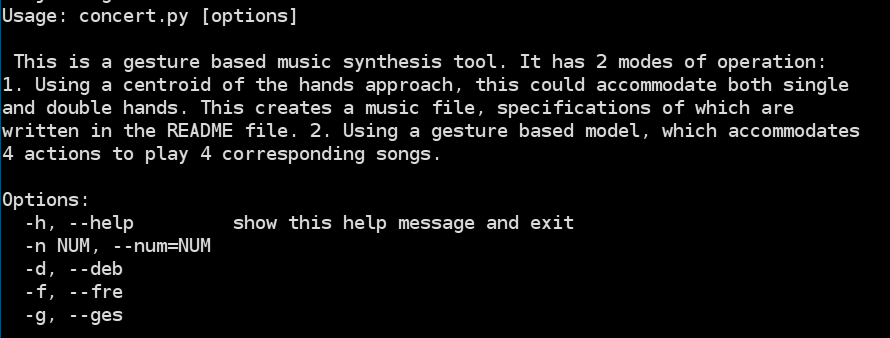
\includegraphics[width=\columnwidth]{concert.png}
  \caption{Overall1}
  \label{Overall1}
\end{figure}
The software was developed with a user friendly interface, allowing the users to provide
options and arguments. The list of options include:
\begin{itemize}
  \item \texttt{--deb}: Used for employing the Debugging mode.
  \item \texttt{--num}: Used for specifying the number of hands.
  \item \texttt{--fre}: Used along with the above option for free music synthesis.
  \item \texttt{--ges}: Used for a 4-class gesture for music selection, disjoint with the
    above 2 methods.
\end{itemize}

\subsection{Feature Processing}
  As mentioned earlier, the system accepts input from a computer webcamera. The following points illustrate
  the processing associated:
  \begin{itemize}
    \item \textit{Free hand movement}: Under this feature, the RGB frame is converted to a Y-Cb-Cr frame. The
      resultant binarized, thresholded image is sent for a contour analysis, following which the 2 largest
      contours are identified. Now, depending upon the user's choice, the program detects one or two of the user's
      hands and computes a unique identifier for music synthesis and pipes it to the music synthesis process. To guide
      the user, the program also draws a grid showing the pitch and octave variations in the x and y directions
      respectively. This mode computes the centroids of the contours and sends it to the music synthesis process.

      The music synthesis process here evaluates the octave and pitch based on % TODO
      and thus concatenates the entire gesture and creates a song, and plays it.
      \par\null\par
    \item \textit{Gesture selection}: Under this feature, the RGB frame is converted to a Y-Cb-Cr frame. The
      resultant binarized, thresholded image is sent for a contour analysis, following which the largest contour
      is identified. After this, a convex hull is fitted over the identified contour, along with the convexity defects.
      Thus, this gives us the information about the vertices of the convex polygon fitted, and the defects,
      which are the points on the contour which lie farthest from the fitted polygon. The main idea of this is
      to find the junctions between the fingers, with which multiple gestures can be idenitified and classified.
      
      However, the convexity defects contain extraneous points than the desired junctions, and hence need filtering,
      based on the distance from the convex hull and the defect, and the angle subtended between two consecutive
      hull vertices at the defect.
      % TODO: Add equation here.

      After having detected the number of junctions in the gesture implied, the gesture is selected and a corresponding
      song is played. Currently, only 4 gestures are made, but due to its geometric rule based nature, it is natural that
      it can be extended to custom gestures as well.

  \end{itemize}
  \begin{figure}[h]
    \centering
    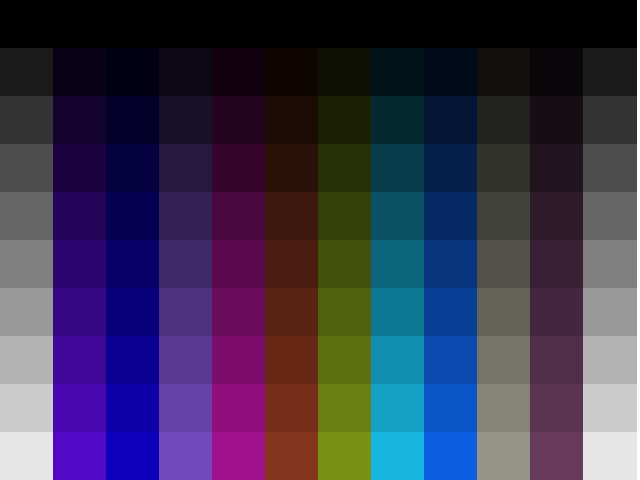
\includegraphics[width=\columnwidth]{wallpaper.png}
    \caption{Overall1}
    \label{Overall1}
  \end{figure}
\subsection{Music Generation}
  The music generation is done using a Python library called Pyknon. The documentation of this library can be found
  in a book written by the writer of this library. The music module is also differentially drafted for each 
  of the above operational modes:
  \begin{itemize}
    \item \textit{Free hand movement}: The music module receives the \texttt{x} and \texttt{y} coordinates
      of the hand centroid. The music module divides the image captured into several blocks in the $X$ and $Y$
      direction. After this, each block represents a certain $(X,Y)$, which corresponds to a certain $(P,O)$,
      where $P$ is pitch and $O$ is octave. This constitutes one single tone.
      Using this concept, the musical objects are sampled over every frame, and the musical tones thus generated are
      concatenated together to form one musical piece. In the end, this piece is synchronously played using
      \texttt{pygame mixers}.
      \par\null\par
    \item \textit{Gesture selection}: The music module receives the gesture ID, and the \texttt{pygame mixer}
      plays the corresponding song from the playlist.
    \end{itemize}
\section{MAJOR HEADINGS}
\label{sec:majhead}

Major headings, for example, "1. Introduction", should appear in all capital
letters, bold face if possible, centered in the column, with one blank line
before, and one blank line after. Use a period (".") after the heading number,
not a colon.

\section{PRINTING YOUR PAPER}
\label{sec:print}

Print your properly formatted text on high-quality, 8.5 x 11-inch white printer
paper. A4 paper is also acceptable, but please leave the extra 0.5 inch (12 mm)
empty at the BOTTOM of the page and follow the top and left margins as
specified.  If the last page of your paper is only partially filled, arrange
the columns so that they are evenly balanced if possible, rather than having
one long column.

In LaTeX, to start a new column (but not a new page) and help balance the
last-page column lengths, you can use the command ``$\backslash$pagebreak'' as
demonstrated on this page (see the LaTeX source below).

\section{PAGE NUMBERING}
\label{sec:page}

Please do {\bf not} paginate your paper.  Page numbers, session numbers, and
conference identification will be inserted when the paper is included in the
proceedings.

\section{ILLUSTRATIONS, GRAPHS, AND PHOTOGRAPHS}
\label{sec:illust}

Illustrations must appear within the designated margins.  They may span the two
columns.  If possible, position illustrations at the top of columns, rather
than in the middle or at the bottom.  Caption and number every illustration.
All halftone illustrations must be clear black and white prints.  Colors may be
used, but they should be selected so as to be readable when printed on a
black-only printer.

Since there are many ways, often incompatible, of including images (e.g., with
experimental results) in a LaTeX document, below is an example of how to do
this \cite{Chai1999}.

\section{FOOTNOTES}
\label{sec:foot}

Use footnotes sparingly (or not at all!) and place them at the bottom of the
column on the page on which they are referenced. Use Times 9-point type,
single-spaced. To help your readers, avoid using footnotes altogether and
include necessary peripheral observations in the text (within parentheses, if
you prefer, as in this sentence).

% Below is an example of how to insert images. Delete the ``\vspace'' line,
% uncomment the preceding line ``\centerline...'' and replace ``imageX.ps''
% with a suitable PostScript file name.
% -------------------------------------------------------------------------
\begin{figure}[htb]

\begin{minipage}[b]{1.0\linewidth}
  \centering
  %\centerline{\includegraphics[width=8.5cm]{image1}}
%  \vspace{2.0cm}
  \centerline{(a) Result 1}\medskip
\end{minipage}
%
\begin{minipage}[b]{.48\linewidth}
  \centering
  %\centerline{\includegraphics[width=4.0cm]{image3}}
%  \vspace{1.5cm}
  \centerline{(b) Results 3}\medskip
\end{minipage}
\hfill
\begin{minipage}[b]{0.48\linewidth}
  \centering
  %\centerline{\includegraphics[width=4.0cm]{image4}}
%  \vspace{1.5cm}
  \centerline{(c) Result 4}\medskip
\end{minipage}
%
\caption{Example of placing a figure with experimental results.}
\label{fig:res}
%
\end{figure}


% To start a new column (but not a new page) and help balance the last-page
% column length use \vfill\pagebreak.
% -------------------------------------------------------------------------
%\vfill
%\pagebreak

\section{COPYRIGHT FORMS}
\label{sec:copyright}

You must submit your fully completed, signed IEEE electronic copyright release
form when you submit your paper. We {\bf must} have this form before your paper
can be published in the proceedings.

\section{RELATION TO PRIOR WORK}
\label{sec:prior}

The text of the paper should contain discussions on how the paper's
contributions are related to prior work in the field. It is important
to put new work in  context, to give credit to foundational work, and
to provide details associated with the previous work that have appeared
in the literature. This discussion may be a separate, numbered Section
or it may appear elsewhere in the body of the manuscript, but it must
be present.

You should differentiate what is new and how your work expands on
or takes a different path from the prior studies. An example might
read something to the effect: "The work presented here has focused
on the formulation of the ABC algorithm, which takes advantage of
non-uniform time-frequency domain analysis of data. The work by
Smith and Cohen  considers only fixed time-domain analysis and
the work by Jones et al  takes a different approach based on
fixed frequency partitioning. While the present study is related
to recent approaches in time-frequency analysis [3-5], it capitalizes
on a new feature space, which was not considered in these earlier
studies."

\vfill\pagebreak

\section{REFERENCES}
\label{sec:refs}

List and number all bibliographical references at the end of the
paper. The references can be numbered in alphabetic order or in
order of appearance in the document. When referring to them in
the text, type the corresponding reference number in square
brackets as shown at the end of this sentence \cite{Chai1999}. An
additional final page (the fifth page, in most cases) is
allowed, but must contain only references to the prior
literature.

% References should be produced using the bibtex program from suitable
% BiBTeX files (here: strings, refs, manuals). The IEEEbib.bst bibliography
% style file from IEEE produces unsorted bibliography list.
% -------------------------------------------------------------------------
\bibliographystyle{IEEEbib}
\bibliography{Template}

\end{document}
